\begin{frame}{Schemat dowodu}

    \begin{figure}
    \centering
        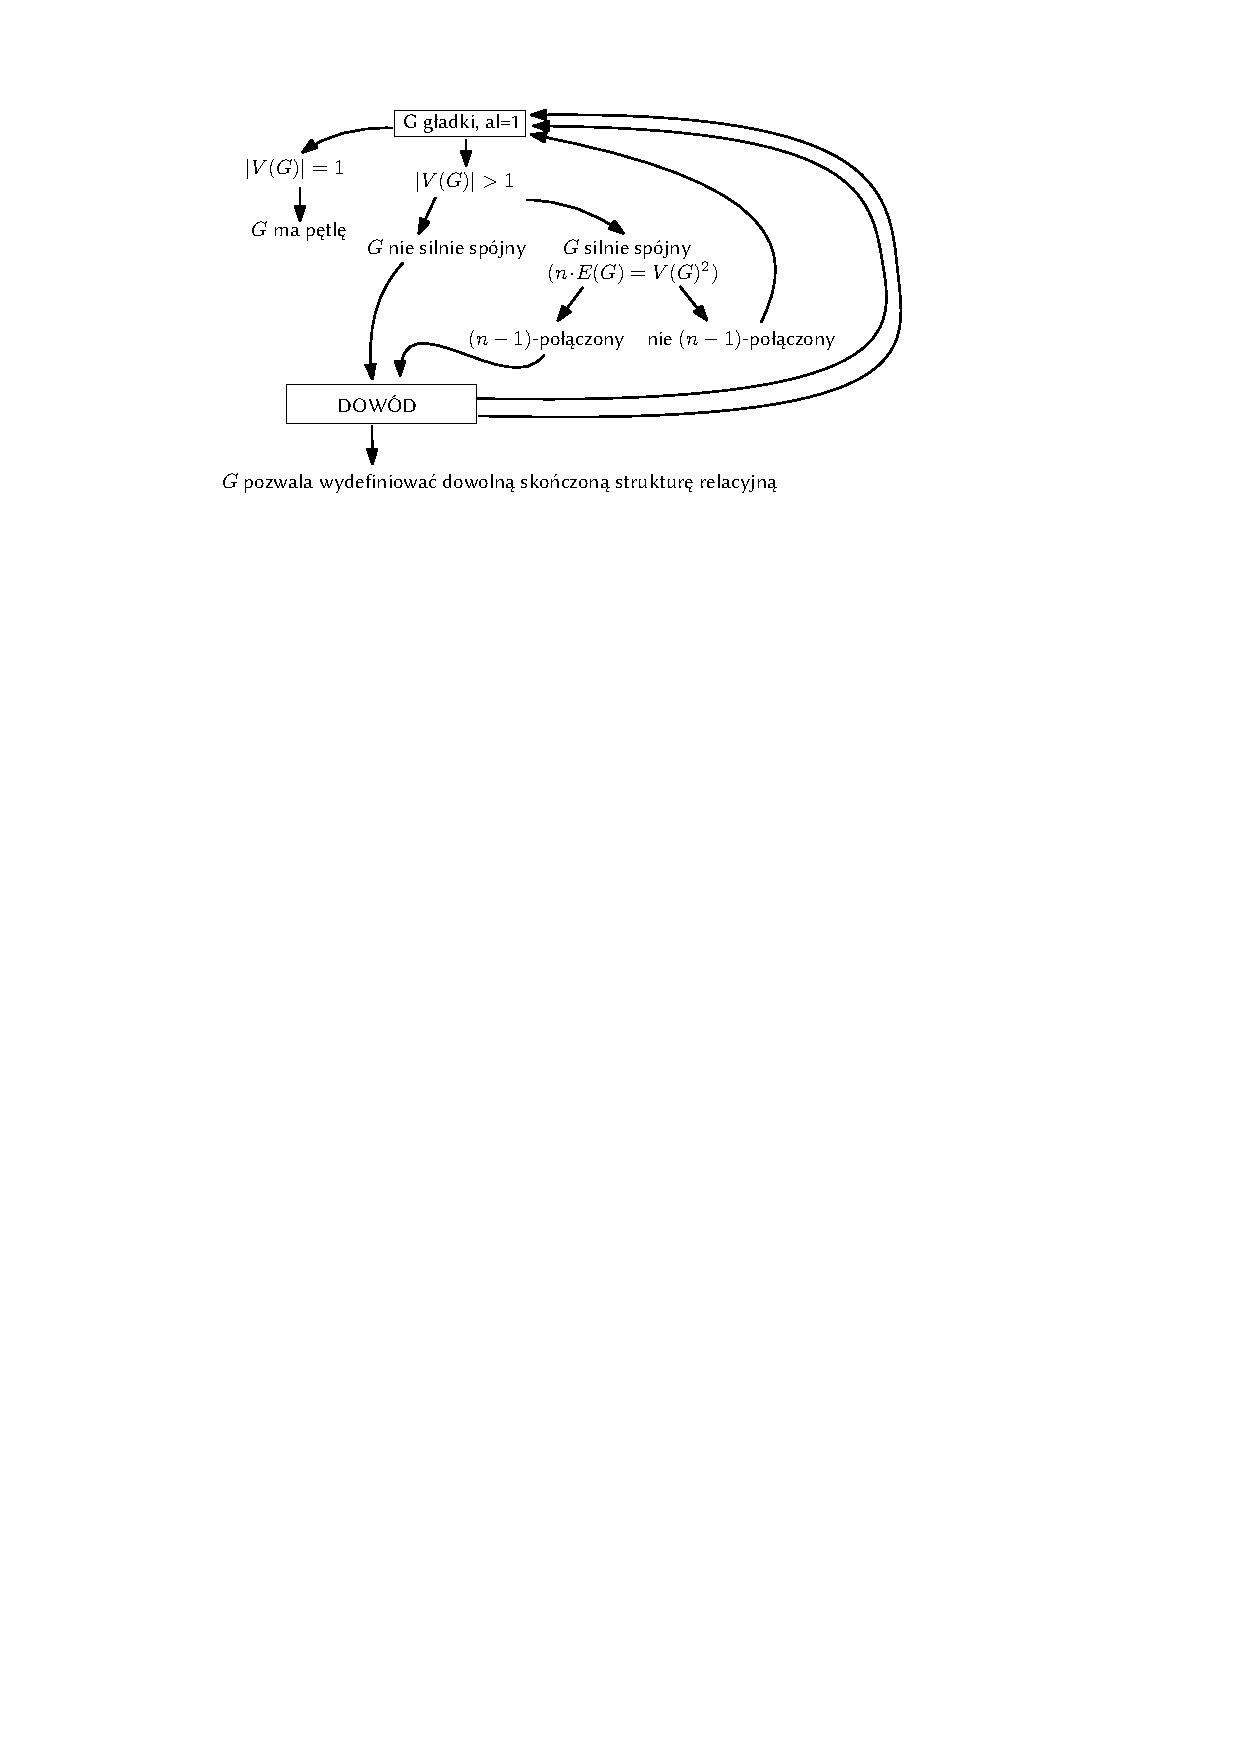
\includegraphics[]{img/proof.pdf}
    \end{figure}

\end{frame}

%---------------------------------------------------------

\begin{frame}[t]{Kroki dowodu indukcyjnego}
    \begin{itemize}
        \item  Na podstawie początkowej relacji \(R\) definiujemy
        \begin{itemize}
            \item relację z nietrywialnym centrum \(R_C(x,y)\)
            \only<1>{\[ C = \set{x: \forall_{v \in V} \ R_C(x,v)} \]
            }
            \item relację z nietrywialną centralną równoważnością \(R_{CE}(x,y,z)\)
            \only<1>{
            \[ \alpha_{\text{CE}} = \set{(x,y): \forall_{v \in V} \ R_{CE}(x,y,v)} \]
            }
        \end{itemize}
        \only<2->{
            \item Definiujemy relację \(\dord\) dla pewnego zbioru \(D\)
            \only<2>{
            \[\dord(x,z) \iff x \in D \lor z \in D\]
            }
            z relacją równoważności \(\alpha \subseteq D \times D\).
        }
        \onslide<3->{
            \item Dla wierzchołków z \(D\) definiujemy relacje \(\eqoreq\)
            \only<3>{
            \vspace{-0.5em}
            \[ \alpha\text{or}\alpha(x, x', z, z') \iff \alpha(x = x') \lor \alpha(z = z') \]
            co na grafie ilorazowym \(G_{/\alpha}\) odpowiada
            \vspace{-0.5em}
            \[ \eqoreq(x, x', z, z') \iff (x = x' \lor z = z') \]
            }
        }
        \onslide<4->{
            \item Relacja \(\eqoreq\) pozwala zdefiniować każdy szablon zawierający koniunkcję i alternatywą. 
        }
    \end{itemize}

\end{frame}
